\section{Replication} \label{sec:repl}
In the following two cases are investigated; Case A where the lead node distributes the file directly to all nodes and Case B where the lead node delegates to another node to generate the next replica, in a more Hadoop like manner. These cases are illustrated in figure \ref{fig:repl}. \\
The time to generate all replicas, can be defined by the number of replicas $k$, the data rate $R$, the size of the file in bits $s$ and computation time $T_{process}$. 

\begin{figure}[H]
    \centering
    \begin{subfigure}{.35\textwidth}
        %\centering
        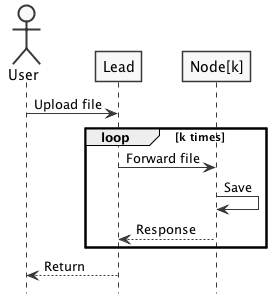
\includegraphics[width=\textwidth]{figures/e2a.png}
        \caption{Case A}
    \end{subfigure}
    \hspace{30px}
    \begin{subfigure}{.42\textwidth}
        %\centering
        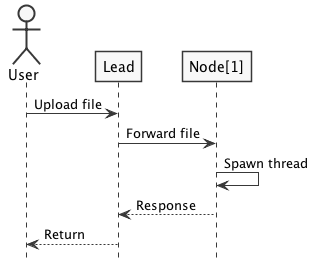
\includegraphics[width=\textwidth]{figures/e2b.png}
        \caption{Case B}
    \end{subfigure}
    \caption{Replication Strategy}
    \label{fig:repl}
\end{figure}

\subsubsection*{Time to generate all replicas}
\textit{Case A:} 
\begin{align} 
    T_{gen} = (k+1)\cdot R\cdot s + T_{process} \label{eq:e2_rep_A}
\end{align}
\textit{Case B:} 
\begin{align}
    T_{gen} = (k+1)\cdot R\cdot s + T_{process} \label{eq:e2_rep_B}
\end{align}

The time to to generate all the replicas for both cases are more or less the same, since the amount of data to be transferred is the same. 

\subsubsection*{Time for lead node to finish}
\textit{Case A:}
\begin{align} 
    T_{lead} = (k+1)\cdot R\cdot s + T_{process} \label{eq:e2_lead_A}
\end{align}
\textit{Case B:}
\begin{align} 
    T_{lead} = 2R \cdot s + T_{process} \label{eq:e2_lead_B}
\end{align}

The lead node is freed earlier in the latter case, given $k > 1$. In this case it only has to send to one other node, instead of $k$.

\subsubsection*{Access time}
\begin{align}
    T_{access} = 2R \cdot s + T_{process}
\end{align}

\subsubsection*{Measurements}
\begin{table}[H]
    \begin{tabularx}{\textwidth}{|X|X|X|X|X|X|}
        \hline
        \cellcolor{lightgray}\textbf{Size} & \cellcolor{lightgray}\textbf{Time Case A [s] (k=2)} & \cellcolor{lightgray}\textbf{Time Case A [s] (k=3)} & \cellcolor{lightgray}\textbf{Time Case B [s] (k=2)} & \cellcolor{lightgray}\textbf{Time Case B [s] (k=3)} & \cellcolor{lightgray}\textbf{Download Time [s]}\\\hline
        10KB  & 0.21    & 0.36   & 0.17   & 0.16   & 0.04  \\\hline
        100KB & 0.46    & 0.48   & 0.18   & 0.20   & 0.18  \\\hline
        1MB   & 1.65    & 2.21   & 1.31   & 1.02   & 0.42  \\\hline
        10MB  & 14.31   & 20.04  & 9.59   & 10.02  & 3.80  \\\hline
        100MB & 144.59  & 203.57 & 109.72 & 111.74 & 37.55 \\\hline
    \end{tabularx}
    \caption{Measurements}
	\label{tab:e2meas}
\end{table}

For Case A, when $k$ increases, it gives a reasonably increase in time, as the lead has to distribute the data to one additional node. As stated in equation \ref{eq:e2_lead_A} which depend on $k$.\\
For Case B, when $k$ increases, there is no significant changes in time, as the lead note, still only have to distribute the data to one other node. As stated in equation \ref{eq:e2_lead_B} which does not depend on $k$.\\
Differences between Case A and Case B. Case A takes longer time for the lead node to be freed, since it has to send the replica to 2 or 3 other, whereas for Case B it always has to only send it to one node.\\
Had Case A been tested with $k=1$ it should give about the same as either Case B, for same file size.